\documentclass{article}

\usepackage[utf8x]{inputenc}
\usepackage[english,russian]{babel}
\usepackage{cmap}
\usepackage{commath}
\usepackage{amsmath}
\usepackage{amsfonts}
\usepackage{mathtools}
\usepackage{amssymb}
\usepackage{parskip}
\usepackage{titling}
\usepackage{color}
\usepackage{hyperref}
\usepackage{cancel}
\usepackage{enumerate}
\usepackage{multicol}
\usepackage{graphicx}
\usepackage[font=small,labelfont=bf]{caption}
\usepackage[a4paper, left=2.5cm, right=1.5cm, top=2.5cm, bottom=2.5cm]{geometry}

\graphicspath{ {./images/} }
\setlength{\droptitle}{-3cm}
\hypersetup{ colorlinks=true, linktoc=all, linkcolor=blue }
\pagenumbering{arabic}

\begin{document}
    \section{Логарифмическая функция и её свойства}

    \subsection{Определения}

    Может оказаться так, что есть \( \mathbb{R} \ni \begin{cases} b_1\qquad\qquad\  a^{c_1}\\ b_2 \xrightarrow[a > 0,\ a \neq 1]{} a^{c_2}\\ b_3\qquad\qquad\  a^{c_3} \end{cases} \), т.к. \( \forall b > 0\ \exists c:\ a^c = b, \) где \( a > 0,\ a \neq 1 \). \( c \) - и есть \(log\).
    
    \textbf{Определение.} Логарифмом числа \(b\) по основанию \(a\) называется такое число \(c\), что \(a^c = b\).

    \(\mathbf{c = \log_a b \Leftrightarrow a^c = b\ (a > 0,\ a \neq 1,\ b > 0)}\)

    \textbf{Свойства:}
    \begin{enumerate}
        \item \(c = \log_a a^c\)
        \item \(a^{\log_a b} = b\)
    \end{enumerate}

    \textbf{Определение.} \(\lg x = \log_{10} x\), десятичный логарифм.
    
    \textbf{Определение.} \(\ln x = \log_e x\), натуральный логарифм.
    
    \subsection{Функция \(y = \log_a x\) и её свойства}
    
    Меняем \( b \Rightarrow \) меняется \(c\); можем рассмотреть \( y = \log_a x \). 

    \(x > 0\quad a > 0,\ a \neq 1\) --- фикс.

    \(y = \log_a x \Leftrightarrow x = a^y \) или в стандартном обозначении \(y = a^x\), т.е. \( y = \log_a x \) --- функция обратная к \( y = a^x \)
    
    \textbf{График.}

    \begin{enumerate}
        \item \(a > 1\)
        
        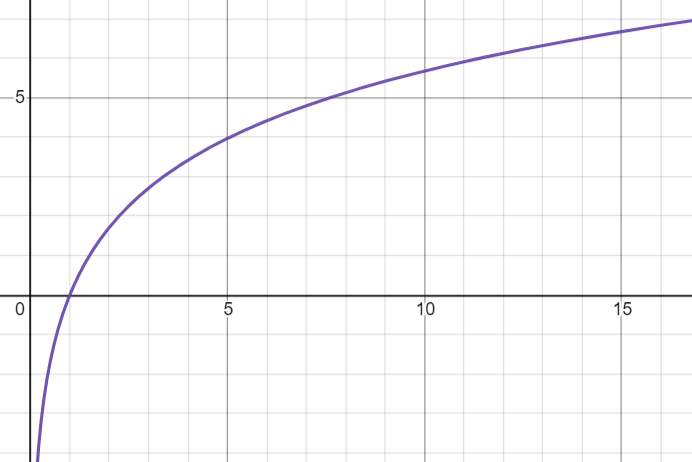
\includegraphics[scale=0.45]{11_1_7_1.png}
        \item \(0 < a < 1\)
        
        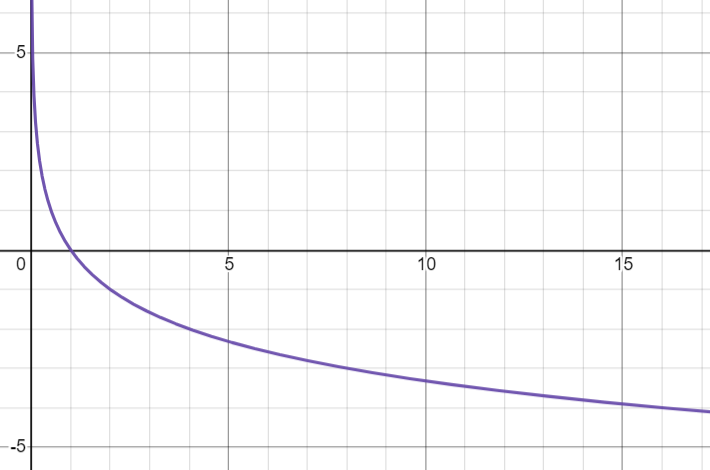
\includegraphics[scale=0.45]{11_1_7_2.png}
    \end{enumerate}

    \textbf{Свойства} \(y = \log_a x, a > 0, a \neq 1\)

    \begin{enumerate}
        \item О.О. \(x > 0\)
        \item О.З. \(y \in \mathbb{R}\)
        \item 
        \begin{enumerate}
            \item \(a > 1\)

            \(\lim_{x \to 0+} \log_a x = +\infty\)

            \(\lim_{x \to +\infty} \log_a x = +\infty\)
            
            \item \(0 < a < 1\)

            \(\lim_{x \to 0+} \log_a x = +\infty\)
            
            \(\lim_{x \to +\infty} \log_a x = -\infty\)
        \end{enumerate}
        \item
        \begin{enumerate}
            \item \( a > 1 \) 
            
            \( \nearrow \)

            \item \( 0 < a < 1 \)
            
            \( \searrow \) 
        \end{enumerate}

        \item Непрерывная как обратная к непрерывной
        \item
        
        \( \log_a 1 = 0 \) 

        \( \log_a a = 1 \)
        
    \end{enumerate}

    \subsection{Операции над log}

    \begin{enumerate}
        \item \(\log_a xy = \log_a x + \log_a y\)

        \( t = \log_a xy \)
        
        \( \alpha = \log_a x \)

        \( \beta = \log_a y \)
        
        \(a^t = xy = a^{\alpha}a^{\beta} = a^{\alpha+\beta} \xLeftrightarrow[]{a \neq 1} t = \alpha + \beta\)

        \textbf{!Замечание!}
        
        О.О. левой части \(xy > 0\)

        О.О. правой части \(x > 0,\ y > 0\)

        \item \( \log_a \frac{x}{y} = \log_a x - \log_a y \)
        
        \( t = \log_a \frac{x}{y} \)
        
        \( \alpha = \log_a x\ a^{\alpha} = x \)

        \( \beta = \log_a y\ a^{\beta} = y \)

        \( a^t = \frac{x}{y} = \frac{a^{\alpha}}{a^{\beta}} = a^{\alpha - \beta} \xLeftrightarrow[]{a \neq 1} t = \alpha - \beta \)
        
        \item \(\log_a x^k = k\log_a x\)
        
        \( t = \log_a x^k \)

        \( \alpha = k\log_a x\ a^{\alpha} = x \)
        
        \(a^t = x^k = (a^\alpha)^k = a^{k \cdot \alpha} \xLeftarrow[]{a \neq 1} t = k \cdot \alpha\)

        \textbf{Примеры.}

        \( \log_a \sqrt{x} = \frac{1}{2}\log_a x (x > 0)\)

        \( \log_a \frac{1}{x} = -\log_a x \)
        
        \item Переход к другому основанию

        \(\log_a b = \frac{\log_c b}{\log_c a} = (\frac{1}{\log_c a})_{\textrm{модуль перехода}}\log_c b\)
    
        \( t = \log_a b \)

        \( \alpha = \log_c a \)
        
        \( \beta = \log_c b \) 
        
        \(a^t = b = c^\beta = (c^\alpha)^\frac{\beta}{\alpha} = a^\frac{\beta}{\alpha} \xLeftrightarrow[]{a \neq 1} t = \frac{\beta}{\alpha} \)
    
        \textbf{Примеры.}
        
        \( \log_a^k b = \frac{1}{k}\log_a b = \frac{\log_a b}{\log_a a^k} = \frac{\log_a b}{k}\)

        \( \log_\frac{1}{a} b = -\log_a b \)
    \end{enumerate}

    \subsection{Второй замечательный предел}
    
    \( \lim_{n \to +\infty} (1 + \frac{1}{n})^n = e \)

    Обобщение

    \(\lim_{x \to \infty} (1 + \frac{1}{x})^x = e\)

    \( x > 0\ \lim_{x \to +\infty} (1 + \frac{1}{x})^x \)

    \(\forall x \in \mathbb{R}\ \exists [x] = n,\ n \in \mathbb{N} \cup \{ 0 \} \)

    т.к. \( x \to +\infty \)\\
    \( 0 < n \leq x < n + 1 \Leftrightarrow \frac{1}{n + 1} < \frac{1}{x} \leq \frac{1}{n} \Leftrightarrow (1 + \frac{1}{n + 1})^n < (1 + \frac{1}{n + 1})^x < (1 + \frac{1}{x})^x \leq (1 + \frac{1}{n})^x < (1 + \frac{1}{n})^{n + 1} \)\\
    \( 1 < (1 + \frac{1}{n + 1})^x \)\\
    \( x \to +\infty \), то \( n = [x] \to +\infty \)
    
    \( \lim_{n \to +\infty}(1 + \frac{1}{n + 1})^n = \lim_{n \to +\infty}\frac{(1 + \frac{1}{n + 1})^{n + 1}}{(1 + \frac{1}{n + 1})} = \frac{e}{1} = e \)\\    
    \(\lim_{n \to +\infty}(1 + \frac{1}{n})^{n+1} = \lim_{n \to +\infty}(1+\frac{1}{n})^n(1+\frac{1}{n}) = e \cdot 1 = e\)

    \(\Rightarrow\) по т. о 2-х милиционерах \(\lim_{x \to +\infty}(1 + \frac{1}{x})^x = e\)

    \(\mathbf{\lim_{x \to -\infty}(1 + \frac{1}{x})^x} = \{ y = -x \} = \lim_{y \to +\infty}(1 - \frac{1}{y})^{-y} = \lim_{y \to +\infty}(\frac{y - 1}{y})^{-y} = \lim_{y \to +\infty}(\frac{y - 1 + 1}{y - 1})^y = \lim_{y \to +\infty}(1 + \frac{1}{y - 1})^y = \lim_{y \to +\infty}(1 + \frac{1}{y - 1})^{y - 1}(1 + \frac{1}{y - 1}) = e(1 + 0) = e \)
    
    \textbf{Следствие.}
    \begin{enumerate}
        \item \(\lim_{u \to 0} (1 + u)^\frac{1}{u} = \begin{cases}
            x = \frac{1}{u}\\
            u = \frac{1}{x}
        \end{cases} = \lim_{x \to \infty}(1 + \frac{1}{x})^x = e\)
        
        \item \((k \neq 0)\ \lim_{x \to \infty}(1 + \frac{k}{x})^x = \{ \frac{x}{k} = y,\ x = ky \} = \lim_{y \to \infty}((1 + \frac{1}{y})^y)^k = (\lim_{y \to \infty}(1 + \frac{1}{y})^y)^k = e^k \)
    
        \item \(\lim_{x \to 0} \frac{\ln(1+x)}{x} = \lim_{x \to 0} \frac{1}{x}\ln(1+x) = \lim_{x \to 0} \ln(1+x)^\frac{1}{x} =_{\textrm{из непрерывности}} \ln(\lim_{x \to 0}(1+x)^\frac{1}{x}) = \ln e = 1\)
        \item \( \lim_{x \to 0}\frac{a^x - 1}{x} = \begin{cases} a^x - 1 = t\\ x \to 0 \Rightarrow t \to 0\\ a^x = t+1\\ x = \log_a(t+1) \end{cases} = \lim_{t \to 0}\frac{t}{\log_a(t + 1)} = \lim_{t \to 0}\frac{1}{\frac{1}{t}\log_a(t + 1)} = \lim_{t \to 0}\frac{1}{\log_a(t + 1)^\frac{1}{t}} = \frac{1}{\log_a e} = \frac{\ln a}{\ln e} = \ln a\)
    \end{enumerate}

    \textbf{Пример.}

    \( \lim_{x \to 0}\frac{\ln(1 + sin(4x))}{5x} \)
\end{document}
